\chapter{Corchetes de \emph{Poisson} vs cuántica}
\label{T20CP}

	
\begin{tikzpicture}
	\fill [left color=red!50, right color=teal!50] (0,0) rectangle (6.5,.1);
	\fill [left color=teal!50, right color=blue!50] (6.5,0) rectangle (11.5,.1);
	\end{tikzpicture}


\vspace{10mm}
\begin{adjustwidth}{50pt}{50pt}
\begin{ejemplo}

Definiremos los corchetes de Poisson, estudiaremos sus propiedades y veremos la intensa relación que guardan con la mecánica cuántica.

\end{ejemplo}
\end{adjustwidth}
\vspace{5mm}
\section{Corchetes de \emph{Poisson}}
\vspace{5mm}


Supongamos que tenemos una función $f(q,p,t)=qp^2+2t$, por ejemplo.

\begin{multicols}{2}
En mecánica hamiltoniana podemos imaginar un espacio formado por las coordenadas $q$ y $p$ llamado \textbf{\emph{espacio de fases}}, de modo que la representación de la $f$ en el espacio de fases da lugar a una curva parametrizada $q(t),\ p(t)$. Pero si además se cumple que $\dot q(t)=\pdv{H}{p}$ y que $\dot p(t)=-\pdv{H}{q}$, entonces esta curva es la curva ``\emph{real}'' del movimiento de un sistema físico. A cada punto de la curva definido por su $q,\ p,\ t$ le corresponderá un valor de $f$. Estamos interesados en saber a qué ritmo cambia $f$ a medida que avanzamos por la curva en el espacio de fases, $\boldsymbol {\dot f}$

\begin{figure}[H]
	\centering
	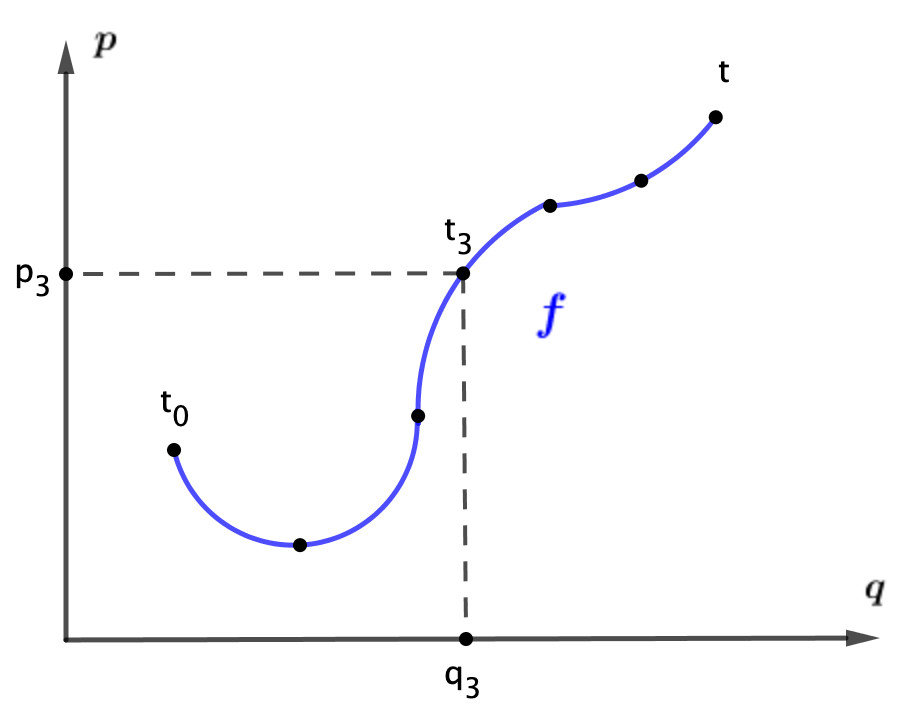
\includegraphics[width=.4\textwidth]{imagenes/img20-01.png}
\end{figure}
\end{multicols}

$\dot f(q,p,t)=\displaystyle \pdv{f}{q} \dot q +\pdv{f}{p} \dot p + \pdv{f}{t}\quad $ Como $\ \displaystyle \dot q(t)=\pdv{H}{p}\ \text{ y } \ \dot p(t)=-\pdv{H}{q}\, , \ $ tendremos

$$\displaystyle \boldsymbol{  \subrayado{ \ 
\dot f \ = \ \pdv{f}{q} \pdv{H}{p} \ - \   \pdv{f}{p} \pdv{H}{q} \ + \ \pdv{f}{t} \ } } $$


En nuestro ejemplo, $f=qp^2+2t$, tendremos $\ \dot f=\displaystyle p^2\pdv{H}{p}-2qp\pdv{H}{q}+2$

Podría ocurrir que tuviésemos un hamiltoniano $H$ tal que $\dot f=0$. Estaríamos ante el curioso caso de tener una función $f$ que dependiendo explícitamente del tiempo $t$ no varíe con el tiempo, $\dot f=0$.

Investigando este tipo de cosas es como Poisson debió darse cuenta de que la expresión $ \pdv{f}{q} \pdv{H}{p}\ -    \pdv{f}{p} \pdv{H}{q}$ aparece con mucha frecuencia y por ello decidiría bautizarla como \emph{\textbf{corchete}}:

\begin{equation}
\label{T20CPdef}
\boldsymbol{
\{A,B\} \ = \  \pdv{A}{q} \pdv{B}{p} \ - \   \pdv{A}{p} \pdv{B}{q}
}	
\end{equation}

Así, la evolución con el tiempo de cualquier magnitud $f$ expresada en el espacio de fases $f(q,p,t)$:

\begin{large}
\begin{equation}
\boxed{ \ 
\boldsymbol{
\dot f \ = \ \{f,H\} \ + \ \pdv{f}{t}
} \ }
\end{equation}
\end{large}

Para más dimensiones, el corchete de Poisson se define como:

\begin{definition}
.	\begin{large}
\begin{equation}
\boxed{ \ 
\boldsymbol{
\{A,B\} \ = \ \sum_{i=1}^n \  \pdv{A}{q_i} \pdv{B}{p_i} \ - \   \pdv{A}{p_i} \pdv{B}{q_i}
} \ }
\end{equation}
\end{large}	
\end{definition}

Con esta definición, Poisson revolucionó la mecánica teórica y, además, abrió las puertas para la mecánica cuántica, la teoría cuántica de campos, etc.

En esta definición está codificada la estructura más profunda de la mecánica teórica más allá de ella misma. Para mostrarlo estudiaremos las propiedades del corchete de Poisson y lo acompañaremos de ejemplos para ver la potencialidad del mismo.

\vspace{5mm} Inciso 1. $\quad$  \rule{150pt}{0.1pt} 

\textbf{ Notación SIMPLÉCTICA} : 

En 1-dim: $\quad z=\mqty(q\\p)\, , \quad $ en n-dim: $\quad z=\mqty(q_1&q_2&\cdots&q_n&\ p_1& p_2& \cdots &p_n)^T\, , \ $ con una transformación canónica, $\quad \mathbb Z=\mqty(Q_1&Q_2&\cdots&Q_n&\ P_1& P_2& \cdots &P_n)^T\, . $

En 1-dim: $\quad \dot z=\mqty(\dot q \\ \dot q) = \mqty( \displaystyle \pdv{H}{p} \\ \displaystyle -\pdv{H}{q} )= J \mqty( \displaystyle \pdv{H}{q} \\ \displaystyle \pdv{H}{p} )=J \displaystyle \pdv{H}{z} \qquad\text{ con } \qquad J=\mqty(0&1\\-1&0)$

En n-dim: $\quad J=\mqty(0&\textcolor{red}{I_{n\times n}} \\ \textcolor{blue}{-I_{n\times n}} &0)\qquad \qquad$
Para 2-dim, $\quad J=\mqty(0&0& \textcolor{red}{1} & \textcolor{red}{0}\\
0&0&\textcolor{red}{0}&\textcolor{red}{1} \\
\textcolor{blue}{-1} & \textcolor{blue}{0}&0&0 \\
\textcolor{blue}{0}&\textcolor{blue}{-1}&0&0 ) $


\begin{flushright}\rule{200pt}{0.1pt}\end{flushright}

Corchete de Poisson en notación simpléctica, para 1-dim:

$\{A,B\} =  \mqty( \displaystyle \pdv{A}{q}&\displaystyle \pdv{A}{p}) \ \mqty ( \displaystyle \pdv{B}{p}\\\displaystyle -\pdv{B}{q}) = \mqty(\displaystyle \pdv{A}{q}&\displaystyle \pdv{A}{p}) \ \mqty(0&1\\-1&0) \ \mqty(\displaystyle \pdv{B}{q} \\ \displaystyle \pdv{B}{p}) =\mqty( \displaystyle \pdv{A}{q}&\displaystyle \pdv{A}{p}) \ J \ \mqty(\displaystyle \pdv{B}{q} \\ \displaystyle \pdv{B}{p})$

\vspace{5mm}
\begin{myblock}{Corchete de Poisson en notación simpléctica}
\begin{large}
\begin{equation}
\label{T20CPenNS}
\boldsymbol{
\{A,B\} \ = \displaystyle \  \left( \pdv{A}{z} \right)^T \ J \ \left( \pdv{B}{z} \right)
}	
\end{equation}	
\end{large}	
\end{myblock}

\vspace{5mm}
\emph{ATENCIÓN}, esta definición válida para $z$, ?`lo es también para $\mathbb Z$, después de efectuar una transformación canónica? Si no lo fuese, la definición anterior no tendría ninguna utilidad, cambiar de $z$ a $\mathbb Z$ lo podemos interpretar como un cambio de sistema de referencia y en física las definiciones han de ser universales, que las fórmulas conservan las forma ante un cambio de sistema de referencia.

\textbf{?`Es $\boldsymbol{ \ \{A,B\} \ }$ invariante bajo transformaciones canónicas?}

Regla de la cadena, $\ \displaystyle \pdv{A}{z}=\pdv{\mathbb Z}{z} \pdv{A}{\mathbb Z}\, ; \ $ dimensionalmente, $\displaystyle \left(\pdv{A}{z}\right)_{2x1}= \left(\pdv{A}{\mathbb Z}\right)_{2x1}  \to \left(\pdv{\mathbb Z}{z}\right)_{2x2}= M\, , \ $ con $\ M=\mqty( \displaystyle \pdv{Q}{q} & \displaystyle \pdv{Q}{p} \\ \displaystyle \pdv{P}{q} & \ \displaystyle \pdv{P}{p})\, , $ por lo que $\ \displaystyle \pdv{A}{z} = M \ \pdv{A}{\mathbb Z} \ \text{ y análogamente } \ \pdv{B}{z} = M \ \pdv{B}{\mathbb Z}$

Trasponiendo, $\ \displaystyle \pdv{A}{z} = M \ \pdv{A}{\mathbb Z} \ \to \left(\pdv{A}{z}\right)^T = \left( M \ \pdv{A}{\mathbb Z} \right)^T = \left( \pdv{A}{\mathbb Z} \right)^T M^T$

Llevando estos resultados a la definición simpléctica de corchetes de Poisson, ec. \ref{T20CPenNS},

$\{A,B\} = \displaystyle \left( \pdv{A}{z} \right)^T \ J \ \left(\pdv{B}{z}\right) = \left( \pdv{A}{\mathbb Z} \right)^T \ M^T\ J \ M\ \left(\pdv{B}{\mathbb Z}\right) = \left( \pdv{A}{\mathbb Z} \right)^T \ J \ \left(\pdv{B}{ \mathbb Z}\right)$
\begin{tiny}\textcolor{gris}{$\quad \mqty(\text{por ser trans. canónica: } \\ M^TJ\ M = J)$}\end{tiny}


Luego, $\displaystyle \boldsymbol{ \left( \pdv{A}{z} \right)^T \ J \ \left(\pdv{B}{z}\right) \ = \ \left( \pdv{A}{\mathbb Z} \right)^T \ J \ \left(\pdv{B}{ \mathbb Z}\right) } \ $ y el corchete de Poisson $\ \{A,B\} \ $ \textbf{sí} es invariante ante una transformación canónica. \hspace{9.5cm} $\Box$


\textcolor{gris}{La importancia de esto junto a las propiedades del corchete de Poisson que veremos a continuación, definirán un Álgebra de Lie\footnote{$\ \ $ https://github.com/igvaori/Grupos-de-Lie/blob/main/GRUPOS-DE-LIE.pdf} (las magnitudes que se conservan dado un H (ó L) forman un álgebra de Lie).}

\vspace{5mm}
\section{Propiedades del corchete de \emph{Poisson}} 
\label{T20CPP}

\begin{enumerate}[P1.- ]
\item  \begin{equation} \subrayado{\boxed{ \ \boldsymbol{ 
	 \{A,B\}\ \ = \ \ -\{B,A\}
	  } \ }}\end{equation}

$\{A,B\} \ \mqty {_{1)} \\ = \\ \,} \ \displaystyle  \left( \pdv{A}{z} \right)^T \ J \ \left(\pdv{B}{z} \right)=
\left[ \left( \pdv{A}{z} \right)^T \ J \ \left(\pdv{B}{z} \right) \right]^T =
 \left( \pdv{B}{z} \right)^T \ J^T \ \left(\pdv{A}{z} \right)
 \  \mqty {_{2)} \\ = \\ \,} $
 
 $\displaystyle =
-  \left( \pdv{B}{z} \right)^T \ J \ \left(\pdv{A}{z} \right)	=
-\{B.A\}$ \hspace{9cm}$\Box$

\begin{itemize}
\item Donde, $1)\quad \displaystyle \left(\pdv{A}{z} \right)^T_{1\times k} J_{k\times k} \left(\pdv{B}{z} \right)_{k\times 1}=\{A,B\}_{1\times 1}= \text{ número } \to \{A,B\}=\{A,B\}^T$

\item Y, $2) \quad J^T=\mqty(0&1\\-1&0)^T=\mqty(0&-1\\1&0)=-J$
\end{itemize}

\vspace{5mm}
\item  \begin{equation} \subrayado{\boxed{ \ \boldsymbol{ 
	 \{\alpha A + \beta B , C\}\ \ = \ \ \alpha\{A,C\} \ + \ \beta \{A,C\}
	  } \ }} \qquad \alpha,\beta = ctes \end{equation}
	  
$\displaystyle \{\alpha A + \beta B, C\} =
 \left[ \pdv{z} (\alpha A + \beta B) \right]^T J \left( \pdv{C}{z} \right)=
\left( \alpha \pdv{A}{z} + \beta \pdv{B}{z} \right)^T J \left( \pdv{C}{z} \right)=$

$\displaystyle =
\left[ \alpha \left(\pdv{A}{z} \right)^T + \beta \left(\pdv{B}{z} \right)^T \right] J  \left(\pdv{C}{z} \right)=
\alpha \left(\pdv{A}{z} \right)^T J \left(\pdv{C}{z} \right) + 
\beta \left(\pdv{B}{z} \right)^T J \left(\pdv{C}{z} \right) =$

$\displaystyle =
\alpha \{A,C\} + \beta \{B,C\} $ \hspace{11cm}$\Box$

\vspace{5mm}
\item  \begin{equation} \subrayado{\boxed{ \ \boldsymbol{ 
	 \{AB,C\}\ = \ A\ \{B,C\} \ + \ \{A,C\}\ B
	  } \ }}  \end{equation}
	  
$\{AB,C\} 
\ \mqty {_{1)} \\ = \\ \,} \
  \left[ \partial (AB)^T \right] J (\partial C) = \left[ (\partial A) B + A(\partial B) \right]^T J (\partial C)
\ \mqty {_{2)} \\ = \\ \,} \
\left[ B (\partial A)^T + A(\partial B)^T \right] J (\partial C)=$

$ = B(\partial A)^T J (\partial C) + A (\partial B)^T J (\partial C)= B \{A,C\} + A\{B,C\}
\ \mqty {_{3)} \\ = \\ \,} \
 A \{B,C\}\ + \{A,C\} B$ \hspace{2.5cm} $\Box$
 
 \begin{itemize}
 \item Donde $1)\quad $ Para mayor comodidad en la demostración, escribiremos el corchete de Poisson en la forma: $\ (\partial A)^T J (\partial B) \ \textcolor{gris}{\ \ \ = \ \displaystyle \left( \pdv{A}{z}\right)^T J \left(\pdv{B}{z}\right)}$ 
 \item $2) \quad A \text { y } B$ son escalares (funciones), $A^T=B,\ B^T=B$
 \item Y $3)\quad $ El resultado sería cierto si $AB=BA$, si las magnitudes conmutasen, pero \emph{puede haber parejas de magnitudes que no conmuten}, que $AB\neq BA$. Para prevenir estos casos, como hemos puesto en el enunciado de la propiedad el producto $AB$, siempre que aparezcan juntas $A$ y $B$ pondremos $A$ a la izquierda, premultiplicando,  y $B$ a la derecha, postmultiplicando.
 \end{itemize}

\vspace{5mm}
\item  \begin{equation} \subrayado{\boxed{ \ \boldsymbol{ 
	\textbf{Identidad de Jacobi } \quad \{\textcolor{red}{A},\{B,C\}\}\ + \ \{C\{\textcolor{red}{A},B\}\} \ + \ \{B,\{C,\textcolor{red}{A}\}\}\
	  } \ }}  \end{equation}
	  
Permutaciones cíclicas $\ A \to B \to C \to A \to B \to \cdots $

La demostración de esta propiedad se deja como ejercicio (al final del tema).

\end{enumerate}

\vspace{5mm}
\begin{ejemplo}
\color{gris}
\begin{small}
Ejercicio para matemáticos: demostrar que para cualquier operación $(A,B)$ definida de modo que cumpla las propiedades 1) a 4) del corchete de Poisson y tal que $AN\neq BA$ (no conmutativa) inexorablemente ha de cumplir que $\ (A,B) \ = \ K\ (AB-BA) \,  , \ $ con $K=cte$.

Este teorema codifica el transito de la mecánica teórica a la mecánica cuántica.

La mecánica teórica, que proviene de Newton, nos conduce al corchete de Poisson con sus cuatro propiedades. A principios del s. XX se inventa en MQ (mecánica cuántica) un sustituto del corchete de Poisson abstracto, llamado $[A,B]$	. Según el teorema anterior, $[A,B]=K(AB-BA)$ que da lugar a la mecánica cuántica a los valores discretos, a que hay que trabajar con operadores autoadjuntos (formalismo de Liouville) que se pueden diagonalizar y dan lugar a una base ortogonal de funciones $\{f_1(x),\ f_2(x);\ \cdots \}$ que tienen asociados unos valores propios $\{ \lambda_1,\ \lambda_2,\ \cdots \}$ que son números reales y que Heissemberg dijo que correspondían con las mediciones (cuántos) de los operadores autoadjuntos (observables). Se vio que la constante del teorema es $k=\dfrac 1{i\hbar}$

\vspace{5mm} Vamos a jugar e inventar una nueva teoría con la ayuda de este teorema.

En mecánica clásica (MC), $\ \{q,p\}=\mqty(\pdv{q}{q}\\ \pdv{p}{p})^T \mqty(0&1\\-1&0) \mqty(\pdv{p}{q} \\ \pdv{p}{p})=\mqty(1\\0)^T \mqty(0&1 \\ -1&0)\mqty(0\\1)=1$

Se pede comprobar que $\ \{q,q\}=0 \ \text{ y } \ \{p,p\}=0$

Estamos interesados en crear una nueva teoría tal que $\ q\to \Box;\ \ p\to \triangle \ \text{ y } \ \{q,p\} \to [\Box, \triangle ]\ $ que cumpla las tres relaciones anteriores: $\quad [\Box, \triangle ]=1(\Box \triangle - \triangle \Box )=1;\ \ [\Box, \Box]=[\triangle, \triangle ]=0$

?`Quienes pueden ser $\Box \text{ y } \triangle$? 

Queremos que sean \emph{operadores lineales} que actúen sobre funciones: $\Box(\lambda f + \mu g)=\lambda \Box f + \mu \Box g$ y lo mismo para $\triangle$.

Una posibilidad sencilla (estamos creando una teoría nueva para probar como funciona esto) podría ser: $\ \Box=\pdv{x} \ \text{ y } \ \triangle=x$. Son operadores lineales:

$\pdv{x}(\lambda f + \mu g)=\lambda \pdv{x} f + \mu \pdv{x} g \ ; \qquad \qquad x(\lambda f + \mu g)=\lambda x f + \mu x g$

Comprobemos que se cumplen las tres relaciones del corchete de Poisson:

--- $\ \ [\Box, \triangle ] f=\Box \triangle f - \triangle \Box f = \pdv{x} (xf)-x\pdv{x}f=(xf)'-xf'=f+xf'-xf'=f \ , \ \  \forall f \to  [\Box, \triangle ] =1$

--- $\ \ [\Box, \Box]f=[\pdv x, \pdv x] f =\pdv[2]{x} f -\pdv[2]{x}f=f''-f''=0$

---$\ \ [\triangle,\triangle ]f=[x,x]f=xxf-xxf=x^2f-x^2f=0$

Con nuestra elección para nuestra teoría, $\ \Box=\pdv{x} \ \text{ y } \ \triangle=x \, \ $ podemos llamar a la energía cinética $T=\dfrac {x^2}{2m}$ y energía potencial a $V=\displaystyle \dfrac k 2 \pdv[2]{x}$ con lo que nuestro operador energía en esta nueva teoría sería $E=\displaystyle \dfrac {x^2}{2m} +\dfrac k 2 \pdv[2]{x} \quad$ 
\begin{footnotesize}
 (por analogía a la MC donde $T=p^2/2m$ y $V=k/2\ x^2$)	
\end{footnotesize}


La transición de MC a MQ se hace con $AB\neq BA$ y trabajando en $\mathbb C$ (no en $\mathbb R$). En MC: $\{q,p\}=1$, al cuantizar la teoría se tiene, en MQ, $[q,p]=-i\hbar$, que en el límite cuando $\hbar \to 0$ reproduce el caso clásico.
\end{small}
\color{black}
\end{ejemplo}






\vspace{10mm}
\section{Ejercicio propuesto}

\vspace{5mm}
\begin{ejercicio}
\begin{adjustwidth}{10pt}{10pt}
Demostrar la identidad de Jacobi:

$$ \{A,\{B,C\}\}\ + \ \{C\{A,B\}\} \ + \ \{B,\{C,A\}\}\ $$


\end{adjustwidth} 	
\end{ejercicio}

\vspace{5pt}

\color{NavyBlue}


$\textbf{Identidad de Jacobi} \qquad \{A,\{B.C\}\} \ + \ \{C,\{A,B\}\} \ + \  \{B,\{C,A\}\} \ = \ 0$

$\text{Corchete de Poisson} \qquad \{A,B\} \ = \ \partial A^T \ J \ \partial B$
 
\vspace{5mm}

$\{A,\{B,C\}\}\ = \{A,\partial B^T J \partial C\}= \partial A^T J \partial ( \partial B^T J \partial C) = \ (\partial J = 0) \ =
\partial A^T J [ \partial \partial B^T J \partial C + \partial B^T J \partial \partial C ] = \partial A^T J \partial \partial B^T J \partial C + \partial A^T J  \partial B^T J \partial \partial C =
\{A,\partial B^T\} J \partial C + \partial A^T J \{B, \partial C\}$

Análogamente, alternando cíclicamente los valores de $A,\ B \text{ y } C$, tenemos:

$\{C,\{A,B\}\}=\{C,\partial A^T\}J \partial B + \partial C^T J \{A, \partial B\} \qquad \text{ y } \qquad \{B\{C,A\}\}\ = \{B,\partial C^T\}J \partial A + \partial B^T J\{C,\partial A\}=$

Sumando estas tres expresiones,

$= \{A,\{B.C\}\} \ + \ \{C,\{A,B\}\} \ + \  \{B,\{C,A\}\} \ = 
\{A,\partial B^T\} J \partial C + \partial A^T J \{B, \partial C\} \ + \    \{C,\partial A^T\}J \partial B + \partial C^T J \{A, \partial B\} \ + \{B,\partial C^T\}J \partial A + \partial B^T J \{C,\partial A\} = $

Reorganizando,

$=\{A, \partial B^T\}J \partial C + \partial  C^T J \{A,\partial  B\} \ + \ 
\{B, \partial  C^T\}J \partial A \ + \ \partial  A^T J \{B, \partial  C\} \ + \ 
\{C, \partial  A^T\} J \partial  B \ + \ \partial B^T J \{C, \partial  A\}
\begin{matrix} _\divideontimes \\ =  \\ \, \end{matrix}$

Como $\partial C^T J \{A, \partial  C\}$ es un número real, coincide con su traspuesto:


$\partial C^T J \{A, \partial  C\}=[\partial C^T J \{A, \partial  C\}]^T=
\{A, \partial B\}^T J^T (\partial C^T)^T = (\to) $

Como $ \{A, \partial B\}^T=\{A, \partial B\}  \text{ por ser un número} ; \ \  (\partial C^T)^T=\partial C;\ \ J^T=-J $, tendremos

$(\to )= \{A,\partial B\} (-J) \partial C =- \{A,\partial B\} J \partial C$ y análogamente para los términos pares de la expresión $\divideontimes$ con lo que podremos escribir,

$\begin{matrix} _\divideontimes \\ =  \\ \, \end{matrix}
\{A, \partial B^T\}J \partial C - \ \{A,\partial B\}J \partial C \ 
+ \ 
\{B, \partial  C^T\}J \partial A \ -\  \{B,\partial C\} J \partial A \ 
+ \ 
\{C, \partial  A^T\} J \partial  B \ + \ \{C,\partial A\} J \partial B
= 
[\{A,\partial B^T\}-\{A,\partial B\}]J\partial C+
[\{B,\partial C^T\}-\{B,\partial C\}]J\partial A+
[\{C,\partial A^T\}-\{C,\partial A\}]J\partial B
\begin{matrix} _\divideontimes \\ =  \\ ^\divideontimes \end{matrix}$

Como $B$ es un escalar, $B=B^T \ \to \ \partial B=\partial B^T \quad \text{y} \quad {\{A,\partial B\}-\{A,\partial B^T\}}=0$ y análogamente para los otros dos cocientes, entonces,

$\begin{matrix} _\divideontimes \\ =  \\ ^\divideontimes \end{matrix}
\ 0\ J\partial C \ + \  0\ J\partial B \ + \  0\ J\partial B\ =\ 0$  \hspace{9.5cm} $\Box$

\rule{250pt}{0.1pt}

\vspace{1cm}

De otro modo,
$\{A,B\} \ = \  \pdv{A}{q} \pdv{B}{p} \ - \   \pdv{A}{p} \pdv{B}{q}
\quad \to \quad
\{A,\{B.C\}\} \ + \ \{C,\{A,B\}\} \ + \  \{B,\{C,A\}\} \ = \ 0$



\vspace{5mm}

$\displaystyle \{A,\{B.C\}\}=\pdv{A}{q} \pdv{p} \{B,C\} - \pdv{A}{p}\pdv{q} \{B,C\} = $

$\displaystyle =
\pdv{A}{q} \pdv{p} \left(\pdv{B}{q} \pdv{C}{p} \ - \   \pdv{B}{p} \pdv{C}{q} \right) - \pdv{A}{p}\pdv{q} \left(\pdv{B}{q} \pdv{C}{p} \ - \   \pdv{B}{p} \pdv{C}{q} \right)=$

\vspace{5mm} 

$=\displaystyle \pdv{A}{q}
\left( \pdv{B}{q}{p} \pdv{C}{p} + \pdv{B}{q} \pdv[2]{C}{p} -\pdv[2]{B}{p}\pdv{C}{q} - \pdv{B}{p} \pdv{C}{q}{p} \right)
-\pdv{A}{p}
\left( \pdv[2]{B}{q}\pdv{C}{q} + \pdv{B}{q}\pdv[2]{B}{q} - \pdv{B}{q}{p} \pdv{C}{q} - \pdv{B}{p}\pdv[2]{C}{q} \right) =$

\vspace{5mm} 
$=\displaystyle 
\ \ \ + \pdv{A}{q} \pdv{B}{q}{p} \pdv{C}{p} +\pdv{A}{q} \pdv{B}{q} \pdv[2]{C}{p} -\pdv{A}{q}\pdv[2]{B}{p}\pdv{C}{q} -\pdv{A}{q} \pdv{B}{p} \pdv{C}{q}{p} \ (\to) $

$\displaystyle (\to) -\pdv{A}{p} \pdv[2]{B}{q}\pdv{C}{p} -\pdv{A}{p} \pdv{B}{q}\pdv{C}{q}{p} +\pdv{A}{p} \pdv{B}{q}{p} \pdv{C}{q} +\pdv{A}{p}\pdv{B}{p}\pdv[2]{C}{q}  =$

\vspace{5mm} 

$\displaystyle =\ \ \  
\cancel{\textcolor{red}{+\pdv{A}{q} \pdv{B}{q} \pdv[2]{C}{p}} } \ +\pdv{A}{p}\pdv{B}{p}\pdv[2]{C}{q} \ \ -\pdv{A}{q}\pdv[2]{B}{p}\pdv{C}{q}  \ \ \cancel{\textcolor{teal}{ -\pdv{A}{p} \pdv[2]{B}{q}\pdv{C}{p} }}
\ \ (\to)
$

$\displaystyle (\to) \ 
+ \pdv{A}{q} \pdv{B}{q}{p} \pdv{C}{p} +\pdv{A}{p} \pdv{B}{q}{p} \pdv{C}{q}  -\pdv{A}{q} \pdv{B}{p} \pdv{C}{q}{p}  \cancel{\textcolor{blue}{-\pdv{A}{p} \pdv{B}{q}\pdv{C}{q}{p} } } =$

\vspace{5mm} 
Analicemos el resultado obtenido y comparemos con los que se obtendrán al permutar cíclicamente los operadores $A,\  B \text{ y } C$

\vspace{5mm} 
$\displaystyle \{C,\{A,B\}\} \ =  \qquad \textcolor{SkyBlue}{[A\to C;\ B\to A;\ C\to B]}$ 

$\displaystyle =\ \ \  
+\pdv{C}{q} \pdv{A}{q} \pdv[2]{B}{p}  \ \cancel{\textcolor{teal}{+\pdv{C}{p}\pdv{A}{p}\pdv[2]{B}{q} }} \ \ -\pdv{C}{q}\pdv[2]{A}{p}\pdv{B}{q}  \ \ -\pdv{C}{p} \pdv[2]{A}{q}\pdv{B}{p} 
\ \ (\to)
$

$\displaystyle (\to) \ 
+ \pdv{C}{q} \pdv{A}{q}{p} \pdv{B}{p} +\pdv{C}{p} \pdv{A}{q}{p} \pdv{B}{q}  -\pdv{C}{q} \pdv{A}{p} \pdv{B}{q}{p}  -\pdv{C}{p} \pdv{A}{q}\pdv{B}{q}{p}   =$



\vspace{5mm} 
$\displaystyle \{B,\{C,A\}\} \ = \qquad \textcolor{SkyBlue}{[A\to B;\ B\to C;\ C\to A]}$

$\displaystyle =\ \ \  
+\pdv{B}{q} \pdv{C}{q} \pdv[2]{A}{p}  \ +\pdv{B}{p}\pdv{C}{p}\pdv[2]{A}{q} \ \ \cancel{\textcolor{red}{-\pdv{B}{q}\pdv[2]{C}{p}\pdv{A}{q} }} \ \ -\pdv{B}{p} \pdv[2]{C}{q}\pdv{A}{p} 
\ \ (\to)
$

$\displaystyle (\to) \ 
 \cancel{\textcolor{blue}{+ \pdv{B}{q} \pdv{C}{q}{p} \pdv{A}{p}}} +\pdv{B}{p} \pdv{C}{q}{p} \pdv{A}{q}  -\pdv{B}{q} \pdv{C}{p} \pdv{A}{q}{p}  -\pdv{B}{p} \pdv{C}{q}\pdv{A}{q}{p}   =$
 
\vspace{5mm}
Sumando las tres expresiones, por cada término que aparece en las dos primeras, aparece su opuesto en las 4 segundas y todos se cancelan, como puede comprobar el lector.

A modo de ejemplo buscamos tres de ellos, $\ \displaystyle \textcolor{red}{+\pdv{A}{q} \pdv{B}{q} \pdv[2]{C}{p}} \ $ , $\ \displaystyle \textcolor{blue}{-\pdv{A}{p} \pdv{B}{q}\pdv{C}{q}{p} } $ $\text{ y } \textcolor{teal}{\displaystyle -\pdv{A}{p} \pdv[2]{B}{q}\pdv{C}{p}}$

\vspace{5mm} Finalmente, $\ \{A,\{B.C\}\} \ + \ \{C,\{A,B\}\} \ + \  \{B,\{C,A\}\} \ = \ 0 $ \hspace{7cm} $\Box$


 
\color{black}






